\documentclass [a4paper] {report}
\usepackage{amsmath,amssymb,amsthm, bm,bbm, graphicx,listings,braket,subfig,titlesec,cleveref,lipsum,mcode,xcolor-patch, textcomp,float,booktabs,siunitx, listings}
\usepackage[authoryear]{natbib}
\usepackage[section]{placeins}
\usepackage[margin=2.2cm]{geometry}
\titleformat{\chapter}{\normalfont\huge}{\thechapter.}{20pt}{\huge \bf}

\DeclareMathOperator*{\argmin}{arg\,min}
\DeclareMathOperator*{\argmax}{arg\,max}
\newcommand{\norm}[1]{\left\lVert #1 \right\rVert}

\begin{document}
	
	\begin{titlepage}
		\begin{center}
			
			\textsc{\LARGE IN4320 Machine Learning}\\[1.25cm]
			
			\rule{\linewidth}{0.5mm}\\[1.0cm]
			{\huge \bfseries Exercises: Multiple Instance Learning }\\[0.6cm]
			\rule{\linewidth}{0.5mm}\\[1.5cm]
			
			\begin{minipage}{0.4\textwidth}
				\begin{flushleft} \large	
					\emph{Author:}\\
					\textsc{Milan Niestijl, 4311728}
				\end{flushleft}
			\end{minipage}
			
			\vfill
			{\large \today}
		\end{center}
	\end{titlepage}
	
	\section*{1. Naive MIL classifier}
	We first implement a naive MIL classifier. To reduce computational costs, the images are first downscaled with a scaling factor of 0.2. The images are next segmented using the Mean Shift algorithm with a width parameter of 30. To verify that the apples are correctly separated from the background, the obtained segments are plotted for a couple of images in figure \ref{segments}.\\\\
	
	\begin{figure}[H]
		\begin{center}
			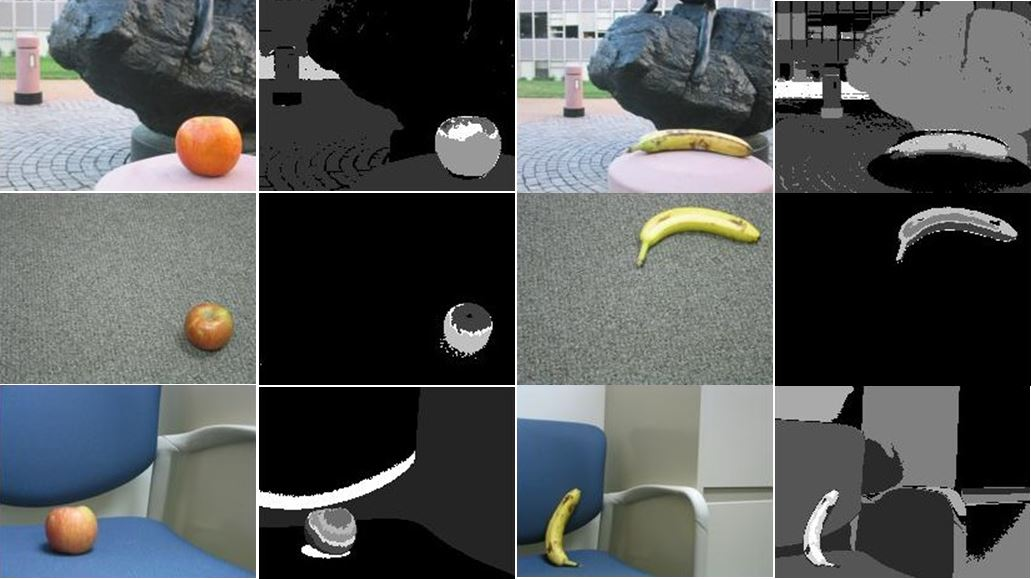
\includegraphics[scale=0.4]{images/segments.jpg}
			\caption{Original and segmented images. One gray scale correspond to a single segment. }
			\label{segments}
		\end{center}
	\end{figure}
	
	Next, a MIL dataset is created using the function \texttt{bags2dataset}. This results in a dataset containing 786 instances belonging to 120 different bags. Thus, on average one bag is segmented in ${786 \over 120} = 5.55$ instances. Each instance has three features; average red, green and blue.
	A scatter plot of the instances can be seen in figure \ref{scatter}. It can be seen that the data is indeed somewhat linearly separable.\\\\
	
	\begin{figure}[H]
		\begin{center}
			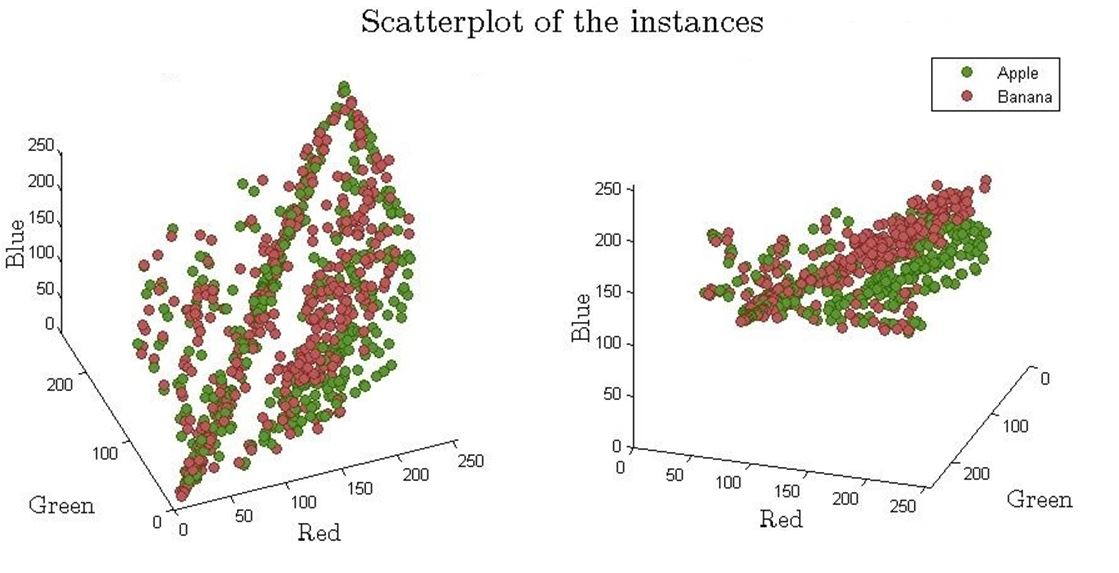
\includegraphics[scale=0.4]{images/scatter.jpg}
			\caption{Scatter plot of all instances from two different perspectives. The label of the instance is copied from the corresponding bag.}
			\label{scatter}
		\end{center}
	\end{figure}
	
	After fitting a linear Fisher classifier on the data, each instance in a bag is classified according to the classifier. The predicted bag label is then decided by majority voting of the instances in the bag. This results in 10 apples being misclassified as a banana and 14 bananas as an apple for a total error of 0.2. This error however, is the training error. More trustworthy would be the test error, which in this case was estimated using a leave-one-out cross-validation strategy. The resulting test error is 0.267. \\
	
	\noindent
	One way to obtain better performance is to include other informative features, for instance by using different statistics regarding the colour (e.g., standard deviation), or adding features that contain information on shape. \\
	
	\noindent
	Secondly, using a different combiner, one that takes the confidence $\mathbb{P}(\bm{y}|\bm{x})$ of the prediction $\bm{y}$ on instance $\bm{x}$ into account would improve the performance. In the implementation above, all instances are weighted equally. However, the Fisher classifier is probabilistic, so the confidence may be used to give a higher weight to instances with a higher confidence. This could significantly reduce the influence that instances corresponding to background have on the final prediction, as they likely have a low confidence.
	
	
	
	\section*{2. MILES}
	Next, the MILES algorithm is implemented. A function embedding a given bag to another representation is implemented. Suppose there are $N$ instances in the training data, denoted by $\bm{x_{i}}$ for $ i=1,2,...N$. Then the embedding $\bm{m}(B)$ of bag $B$ is given by:
	$$ \bm{m}(B) = \left[ s(B,\bm{x_{1}}),s(B,\bm{x_{2}}), ..., s(B,\bm{x_{N}}) \right] $$
	Where 
	$$ s(B,\bm{x_{i}}) = \max_{y\in B} \exp\left(- {\| \bm{y}-\bm{x}\|^{2} \over \sigma^{2}}\right) $$
	For some width parameter $\sigma$. An implementation in Matlab is shown below.
	
	\begin{lstlisting}
	function features = bagembed(bag, data,sigma)
		% Define functions
		K = @(x,y) exp(-norm(x-y)^2/(sigma^2));
		s = @(Bi,y) max(arrayfun(@(j) K(Bi(j,:),y), 1:size(Bi,1)));
		
		% Calculate feature vector
		features = arrayfun(@(j) s(bag,data(j,:)),1:size(data,1));
	end
	\end{lstlisting}
	
	\noindent
	The size of a feature vector is thus equal to the number of training instances. In the apple-banana problem, its size would therefore be 786.\\
	In our case, $\sigma=20$ was used. Next, the embedded feature vectors $\bm{m}(B_{i})$ are stored in a matrix $M$ of size 120-by-786. A Prtools dataset is created using the matrix M and the corresponding bag labels, on which a $L_{1}-$support vector classifier can now be trained. A trade-off parameter $C=10$ was used:
	\begin{lstlisting}
	A = prdataset(M,labels);
	W = liknonc(A,C);
	\end{lstlisting}
	
	\noindent
	 Again using leave-one-out cross-validation, the resulting error on the apple-banana dataset is 0.042. This is clearly a better performance than the naive classifier implemented previously. The algorithm may possibly be further improved by using some (sparse) non-linear classifier. Alternatively, more features could be engineered to capture more information such as, say, shape.

	\newpage
	\section*{3. Other MIL classifiers}
	Finally, we implement a few different MIL classifiers. The full code can be found in the appendix. \\\\
	In order to compare the LIKNON used in MILES with different classifiers, both a Fisher and a K-Nearest Neighbor classifier are fit on the same embedded bag representation that was used in MILES. This was implemented using the functions \texttt{fisherc(X)} and \texttt{knnc(X,k)} in PrTools. After trying various values for the parameter $k$ (for KNN), a value of $k=5$ was found to be best.\\\\
	Secondly, these classifiers (including LIKNON) are also fit on a different bag representation which is based on a bag dissimilarity measure $d$. A symmetric matrix $D$ is computed containing the distances between the bags based on the dissimilarity measure $d$. Two different measures are used. Firstly, the Hausdorff distance $d_{H}$ given by
	$$ d_{H}(A,B) = \max \{\max_{a\in A} \min_{b\in B} \|a-b\|, \max_{b\in B} \min_{a\in A} \|a-b\| \} $$
	and secondly, the minimal distance, given by
	$$ d_{min}(A,B) = \min_{a \in A} \min_{b \in B} \|a-b\| $$
	are used. \\
	The implementation of $d_{H}$ in Matlab is shown below:
	\begin{lstlisting}
	function d = hausdorffDist(A, B)
		d = max(helper(A,B), helper(B,A));
	end
	
	function val = helper(A, B)
		val = max(arrayfun(@(ai) min(arrayfun(@(bj) norm(A(ai,:)-B(bj,:)),1:size(B,1))),1:size(A,1)));
	end
	\end{lstlisting}
	Similarly, for $d_{min}$:
	\begin{lstlisting}
	function d = minDist(A, B)
		d = min(arrayfun(@(ai) min(arrayfun(@(bj) norm(A(ai,:)-B(bj,:)),1:size(B,1))),1:size(A,1)));
	end
	\end{lstlisting}
	A dataset is created using the matrix $D$ and the corresponding labels, on which the various classifiers may now be trained.\\\\
	Using the leave-one-out cross-validation, the resulting performances on the apple-banana dataset are summarized in table \ref{scores}. Note that $M$ corresponds to the feature matrix used in the MILES algorithm.
	
	\begin{table}[H]
		\centering
		\caption{Test error for several classifiers using various embeddings.}
		\label{scores}
		\begin{tabular}{l|lll}
				   & $M$   & $D_{H}$                    & $D_{min}$                  \\ \hline
			LIKNON & 0.042 & 0.242                      & 0.400                     \\
			Fisher & 0.108 & 0.4750                     & 0.533                     \\ 
			5-NN   & 0.208 & 0.4500 					& 0.308 \\
		\end{tabular}
	\end{table}
	
	\noindent
	We conclude that the bag dissimilarity at best performs slightly better than the naive algorithm. This is not surprising, as the instances corresponding to background can have considerable impact on the dissimilarly. For example, the distance between two images with (nearly) the same background is very small, regardless of whether or not they both contain the same fruit. Therefore, the dissimilarity may not at all be representative of whether or not the images contain the same fruit. \\
	However, in the embedding used in the MILES algorithm, a dissimilarity to all instances is computed, allowing an algorithm to give a higher weight to certain instances. This explains the clear performance difference.\\
	Lastly, it can be seen that the Fisher algorithm performs considerably better than the naive one, which is again readily explained by the embedding. 
	
	\newpage
	\section*{Appendix: Code}
	Note: Matlab 2013b was used.\\\\
	\textbf{Read Images:}
	\begin{lstlisting}
function images = openImages( folder, varargin )
% Open all images from given directory. 
% Optional argument: Downsize scaling parameter
% Supported formats: .jpg
	
	% Add trailing '/' if necessary
	if (folder(end) ~= '\') && (folder(end) ~= '/')
		folder = strcat(folder, '/');
	end
	
	% Determine scaling parameter
	if length(varargin)==1
		scale = varargin{1};
		else
		scale = 1;
	end
	
	%% Read images
	content = dir(strcat(folder,'*.jpg'));
	nImgs = length(content);
	
	% load first image to determine the size of the images
	image = readImage(strcat(folder,content(1).name), scale);
	[m,n,d] = size(image);
	images = uint8(zeros(nImgs, m,n,d));
	images(1,:,:,:) = image;
	
	% load the rest of the images
	for j=2:nImgs
		filename = content(j).name;
		images(j,:,:,:) = readImage(strcat(folder,filename), scale);
	end	
end
	
function image = readImage(filename, scale)
	image = imread(filename);
	if scale~=1
	image = imresize(image,scale);
	end
end
	\end{lstlisting}
	
	\newpage
	\noindent
	\textbf{Extract instances:}
	
	\begin{lstlisting}
function features = extractInstances( image, width, varargin)
% Segments an image using the Mean Shift algorithm, computes the average
% red, green and blue color per segment and returns the resulting features
% in a small data matrix
% if optional argument is provided, the segments are plotted.

	segments = uint8(im_meanshift(image, width));
	nSegments = max(max(segments));
	
	% get averages
	features = zeros(nSegments, 3);
	for i=1:nSegments
		features(i,:) = getSegmentAverages(image, segments, i); 
	end

	%% Plot the segments
	if ~isempty(varargin)
		imshow(segments, [1,nSegments]);
		disp(nSegments);
	end
end

function averages = getSegmentAverages(image,segments,targetSegment)
	redIm = image(:,:,1);
	greenIm = image(:,:,2);
	blueIm = image(:,:,3);
	
	red = mean(redIm(segments==targetSegment));
	green = mean(greenIm(segments==targetSegment));
	blue = mean(blueIm(segments==targetSegment));
	
	averages = [red, blue, green];
	end
	\end{lstlisting}
	
	\newpage
	\noindent
	\textbf{Generate apple-banana MIL dataset:}
	
	\begin{lstlisting}
function [bags, labels, MILdataset] = gendatmilsival()
	% creates a MIL dataset using the apples and banana images.
	
	%% Settings
	width = 30;
	scale = 0.2;
	dataset_dir = 'Insert path';
	apple_label = 1;
	banana_label = 2;
	
	%% Load data
	apple_path = strcat(dataset_dir, '\apple');
	banana_path = strcat(dataset_dir, '\banana');
	appleImgs = openImages(apple_path, scale);
	bananaImgs = openImages(banana_path, scale);
	
	nApples = size(appleImgs,1);
	nBananas = size(bananaImgs,1);
	nImgs = nApples + nBananas;
	
	bags = cell(nImgs,1);   
	labels = uint8(ones(nImgs,1)*apple_label);
	labels(nApples+1:nImgs) = banana_label;
	
	%% Extract Instances
	for i=1:nApples
	bags{i} = extractInstances(squeeze(appleImgs(i,:,:,:)), width);
	end
	for i=1:nBananas
	bags{nApples+i} = extractInstances(squeeze(bananaImgs(i,:,:,:)),width); 
	end
	
	MILdataset = bags2dataset(bags, labels);
end
	\end{lstlisting}

	\noindent
	\textbf{Combine labels}
	\begin{lstlisting}
function label = combineinstlabels(labels , rule, varargin)
% Supported rules:
% 'majority' - majority voting
% 'one' - at least one positive
	classes = unique(labels);
	
	%% Perform combining
	if length(classes)==1
		label=classes(1);
	elseif strcmp(rule, 'majority')
		if sum(labels==classes(1))< sum(labels==classes(2))
			label = classes(2);
		else
			label = classes(1);
		end	
	end
end	
	\end{lstlisting}
	
	\newpage
	\noindent
	\textbf{Naive MIL Classifier: Analysis}
	\begin{lstlisting}
function error = analyseNaiveMIL(MILdataset,labels)
% Perform a naive MIL classification on the MILdataset using a Fischer
% classifier and analyse the result.

	%% Definitions
	data = getdata(MILdataset);
	nLab = getnlab(MILdataset);
	milbag = struct(MILdataset).ident.milbag;
	bagIds = unique(milbag);
	N = length(bagIds);
	Kfold = 120;
	
	%% Cross-validation
	indices = crossvalind('KFold',N,Kfold);
	error = zeros(1,Kfold);
	for i=1:Kfold
		testBags = bagIds(indices==i);
		
		% Training 
		trainMask = arrayfun( @(k) ~ismember(milbag(k), testBags),(1:size(MILdataset,1))');
		trainLab = nLab(trainMask);
		train = prdataset(data(trainMask,:),trainLab);
		W = fisherc(train);
		
		% Testing
		testLabels = labels(testBags);
		predictions = zeros(length(testBags),1);
		for b=1:length(testBags)
			testInstances = data(arrayfun(@(k) milbag(k), 1:size(data,1))==testBags(b),:);
			predLabels = testInstances*W*labeld;
			predictions(b) = combineinstlabels(predLabels, 'majority');
		end
		error(i) = mean(predictions ~= testLabels);
	end
end
	\end{lstlisting}
	
	\noindent
	\textbf{Get MILES feature matrix}
	
	\begin{lstlisting}
function M = getFeatureMatrix( MILdataset, sigma )
%% Create feature matrix
	data = getdata(MILdataset);
	nBags = max(struct(MILdataset).ident.milbag);
	M = zeros(nBags, size(data,1));
	for i=1:nBags
		instances = findident(MILdataset,i, 'milbag');
		bag = data(instances,:);
		M(i,:) = bagembed(bag,data,sigma);
	end
end
	\end{lstlisting}
	
	\newpage
	\noindent
	\textbf{Bag distances}
	\begin{lstlisting}
function distances = bagEmbedDist(bag,bags,varargin)
% Compute distance of bag to bags using some bag distance.
% Default distance: Hausdorff
	dist = @(A,B) hausdorffDist(A,B);
	if ~isempty(varargin)
		dist=varargin{1};
	end
	distances = arrayfun(@(i) dist(bag,bags{i}), 1:size(bags,1));
end
	\end{lstlisting}
	
	\noindent
	\textbf{Distance matrix}
	\begin{lstlisting}
function D = distMatrix( bags, varargin )
% Compute distance between bags and store in matrix D.
% Default distance: Hausdorff
	dist = @(A,B) hausdorffDist(A,B);
	if ~isempty(varargin)
		dist=varargin{1};
	end
	N = size(bags,1);
	D = zeros(N,N);
	for i=1:N
		D(i,:) = bagEmbedDist(bags{i},bags,dist);
	end
end


	\end{lstlisting}
	
	\noindent
	\textbf{Split data in test/training datasets.}
	\begin{lstlisting}
function [train, test] = splitData( trainInds, testInds, M, labels, varargin)
% get the score on test bags using a MILES classifier trained on the
% training bags. A proper subset of the feature matrix M is used in
% training/testing.
%
% INPUT:
% TrainInds: Indices of bags to be used as training
% TestInds: Indices of bags to be used as testing
% M: Feature matrix on complete dataset (both training and testing).
% labels: labels of the bags
% milBag(OPTIONAL): array containing the corresponding bag for each feature.
%
% OUTPUT:
% train and test prdataset.

	%% definitions
	ix = 1:size(M,1);
	milBag = 1:size(M,2);
	if length(varargin)==1
	milBag = varargin{1};
	end
	
	%% separate data
	Mtrain = M(ismember(ix, trainInds),ismember(milBag, trainInds));
	trainLabels = labels(ismember(ix, trainInds));
	train = prdataset(Mtrain, trainLabels);
	
	Mtest = M(ismember(ix, testInds),ismember(milBag, trainInds));
	testLabels = labels(ismember(ix, testInds));
	test = prdataset(Mtest, testLabels);
end
	\end{lstlisting}
	
	\newpage
	\noindent
	\textbf{Compare various classifiers}
	\begin{lstlisting}
function scores = compareClassifiers(bags, labels, MILdataset)
% Computes the mean and std scores of various classifiers.
	N=length(labels);

	%% Settings
	Kfold = N;                      %  K-fold cross-validation
	sigma = 20;                     % MILES width parameter
	C = 1;                          % MILES regularization parameter
	classifiers1 = {@(X) liknonc(X,C), @(X) fisherc(X),@(X) knnc(X,5)};
	distFunc = @(A,B) hausdorffDist(A,B);
	
	%% Definitions
	nClassifiers = length(classifiers1);
	
	%% Get feature matrices
	disp('Calculating feature matrices');
	M = getFeatureMatrix(MILdataset, sigma);
	D = distMatrix(bags,distFunc);
	
	%% Perform cross validation
	result = zeros(nClassifiers,2,Kfold);
	indices = crossvalind('KFold',N,Kfold);
	fprintf('\nPerforming %i fold cross-validation\n\n', Kfold);
	for i=1:Kfold
		if mod(i,5)==0
			disp(i)
		end
		trainInds = find(indices~=i);
		testInds = find(indices==i);
		for k=1:nClassifiers
			milbag = struct(MILdataset).ident.milbag;
			[train1, test1] = splitData(trainInds,testInds,M,labels, milbag);
			W1 = classifiers1{k}(train1);
			result(k,1,i) = 1-testd(test1,W1);
			
			[train2, test2] = splitData(trainInds,testInds,D,labels);
			W2 = classifiers1{k}(train2);
			result(k,2,i) = 1-testd(test2,W2);
		end
	end
	
	%% Summarize result
	scores = zeros(nClassifiers,2);
	for i=1:nClassifiers
		scores(i,1) = mean(result(i,1,:));
		scores(i,2) = mean(result(i,2,:));
	end
end
	\end{lstlisting}
	
	\newpage
	\noindent
	\textbf{Plot instances}
	\begin{lstlisting}
function plotInstances( MILdataset, labels, varargin )
	% It is assumed that there are 2 classes, and that the feature space is 3
	% dimensional.
	% optinal input: indices of instances to be highlighted.
	
	set(0,'defaulttextinterpreter','latex')
	
	instances = getdata(MILdataset);
	ident = struct(MILdataset).ident.ident;
	milbag = struct(MILdataset).ident.milbag;
	classes = unique(labels);
	x1 = instances(ident(arrayfun(@(i) labels(i),milbag)==classes(1)),:);
	x2 = instances(ident(arrayfun(@(i) labels(i),milbag)==classes(2)),:);
	disp(length(x1)+length(x2))
	disp(size(instances,1))
	
	figure(1);
	hold on;
	scatter3(x1(:,1), x1(:,2), x1(:,3),'o', 'filled', 'MarkerEdgeColor', ...
		1./255.*[54, 107, 13], 'MarkerFaceColor',  1./255.*[94, 147, 53]);
	scatter3(x2(:,1), x2(:,2), x2(:,3),'o', 'filled', 'MarkerEdgeColor',...
		 1./255.*[136, 47, 47], 'MarkerFaceColor',  1./255.*[186, 87, 87]);
	if ~isempty(varargin)
		x3 = instances(varargin{1},:); 
		scatter3(x3(:,1), x3(:,2), x3(:,3),'o', 'LineWidth', 3, 'MarkerEdgeColor', 1./255.*[255, 191, 0]);
	end
	hold off
	axis([0 255 0 255 0 255])
	legend('Apple', 'Banana');
	xlabel('Red','fontsize', 15);
	ylabel('Green','fontsize', 15);
	zlabel('Blue','fontsize', 15);
	title('Scatterplot of the instances','fontsize', 20)
end
	\end{lstlisting}
	
		

\end{document}